% Poster copy of the report's Fig. 1 (closest unseen holdout reply, tvh-mc3-bottleneck).
% Build: pdflatex fig1_mc3.tex  ->  copy fig1_mc3.pdf to ../figures/
\documentclass[border=2pt]{standalone}
\usepackage[T1]{fontenc}
\usepackage{lmodern}
\usepackage{xcolor,tikz}
\usetikzlibrary{arrows.meta}
\definecolor{tagc}{HTML}{2A78D6}
\definecolor{hiec}{HTML}{EB6834}
\newcommand{\demofont}{\fontsize{5.6}{6.3}\selectfont\ttfamily}
\tikzset{fx/.style={draw, rounded corners=1.5pt, font=\fontsize{5.4}{6}\selectfont, inner sep=1.4pt,
  minimum height=3.6mm, minimum width=6.5mm, fill=white},
  ar/.style={-{Stealth[length=3pt]}, line width=0.4pt}}
\begin{document}
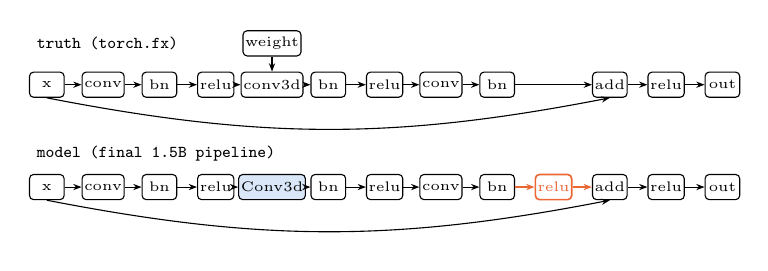
\begin{tikzpicture}[x=7.15mm, y=5mm, sm/.style={fx, font=\fontsize{4.9}{5.5}\selectfont, inner sep=0.8pt, minimum width=4.4mm, minimum height=3.2mm}]
\node[font=\demofont, anchor=west] at (-0.35,1.05) {truth (torch.fx)};
\foreach \i/\l in {0/x,1/conv,2/bn,3/relu,4/conv3d,5/bn,6/relu,7/conv,8/bn,10/add,11/relu,12/out}
  \node[sm] (t\i) at (\i,0) {\l};
\node[sm] (tw) at (4,1.05) {weight};
\foreach \a/\b in {0/1,1/2,2/3,3/4,4/5,5/6,6/7,7/8,8/10,10/11,11/12} \draw[ar] (t\a) -- (t\b);
\draw[ar] (tw) -- (t4); \draw[ar] (t0.south) to[bend right=11] (t10.south);
\node[font=\demofont, anchor=west] at (-0.35,-1.75) {model (final 1.5B pipeline)};
\foreach \i/\l in {0/x,1/conv,2/bn,3/relu,5/bn,6/relu,7/conv,8/bn,10/add,11/relu,12/out}
  \node[sm] (m\i) at (\i,-2.6) {\l};
\node[sm, fill=tagc!18] (m4) at (4,-2.6) {Conv3d};
\node[sm, draw=hiec, text=hiec, line width=0.6pt] (m9) at (9,-2.6) {relu};
\foreach \a/\b in {0/1,1/2,2/3,3/4,4/5,5/6,6/7,7/8,10/11,11/12} \draw[ar] (m\a) -- (m\b);
\draw[ar, draw=hiec, line width=0.6pt] (m8) -- (m9); \draw[ar, draw=hiec, line width=0.6pt] (m9) -- (m10);
\draw[ar] (m0.south) to[bend right=11] (m10.south);
\end{tikzpicture}
\end{document}
